\chapter{Fallstudien}\label{scenarios}
Beim Überführen eines 3D Modells eines Gebäudes in einen Bauplan von einzelnen, sinnvoll platzierten Bausteinen \dots
\section{Modellierung und Bauplandeduktion eines einfachen vierwändigen Turmes mit Anwenden unterschiedlicher Mauerwerksverbände}\label{scenarios:scenario1}
\subsection*{Beschreibung}
In dieser Fallstudie soll ein einfaches, turmartiges Gebäude modelliert werden.
Dies soll mit Hilfe der in Kapitel~\ref{basics} näher behandelten Technologien geschehen und enstpricht darum in seiner Struktur einem verbreiteten Industriestandard.
Das Gebäude besteht lediglich aus vier 20 Meter hohe Wänden, die einen einzigen Raum einschließen.
Es hat einen Grundriss von 10$\times$10 Metern.
Die Wände sollen nun unter Anwendung folgender Mauerwerksverbände realisiert werden:
\begin{itemize}
  \item Einem Läuferverband mit einem Versatz von 50\% der Bausteinlänge.
  \item Einem mittlerern Läuferverband mit einem Versatz von 25\% der Bausteinlänge.
  \item Einem Kopf/Binderverband.
  \item Einem Kreuzverband 
\end{itemize}
Da die beiden letzten Verbände bei gleichbleibendem Modul die Wanddicke verdoppeln, muss das Modell etwas angepasst werden, um nach wie vor den selben Grundriss aufzuweisen.
Als Basismodul wird ein Baustein mit den Maßen 2$\times$1$\times$0.5 Metern verwendet.
Das vereinfacht die Interpretation der generierten Lösungen.

TODO: Bilder, Modelle erstellen, Eckpläne noch einpflegen

\subsection*{Problemstellungen}
Durch Lösen dieser Szenarien sollen folgende Fragestellungen beantwortet werden:
\begin{itemize}
  \item In welcher Art muss das Basismodul vorliegen?
  \item Wie können einem Algorithmus die verschiedenen Mauerwerksverbände sinnvoll übergeben werden?
  \item Wie können Eckbereiche gefunden und der jeweilige Mauerwerksverband auch an diesen stellen passend angebracht werden ohne das Überbindemaß (siehe Kapitel~\ref{basics:Mauerwerksverband}) zu verletzen?
  \item Welche Informationen werden in den resultierenden Bauplan integriert?
\end{itemize}

\section{Modellierung und Bauplandeduktion eines LEGO Gebäudes mit Einsteinmauerwerk}\label{scenarios:scenario2}
\begin{figure}[ht]
  \begin{subfigure}[b]{0.44\columnwidth}
    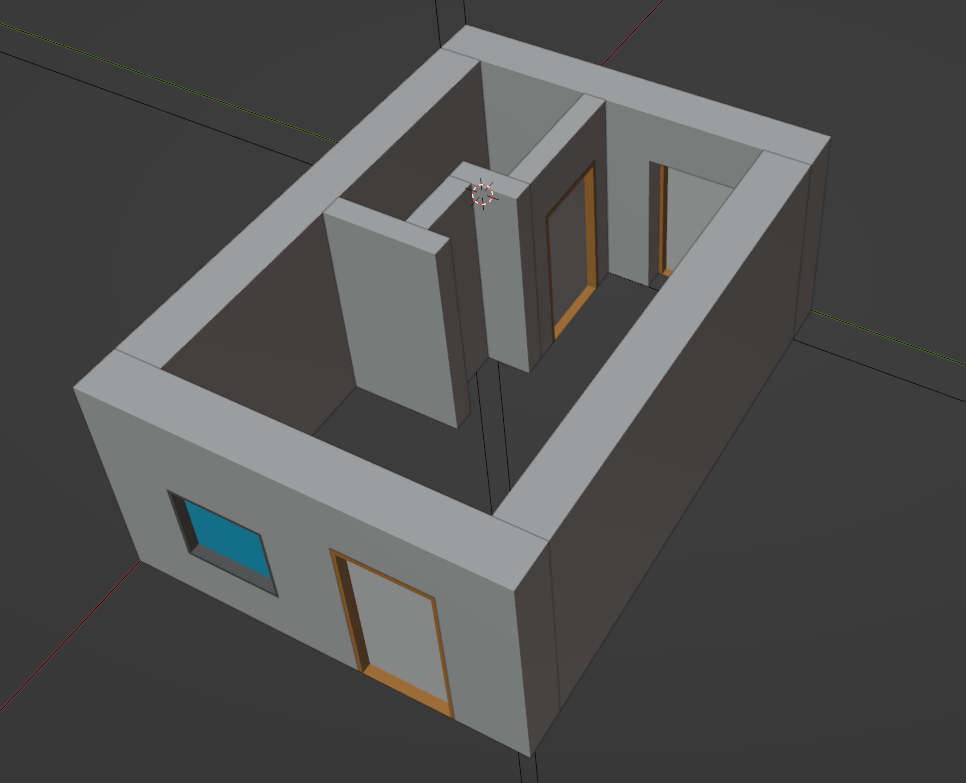
\includegraphics[width=\columnwidth]{fig/scenario1_screenshot.png}
    \caption{3D Modell innerhalb von Blender.}
    \label{fig:Scenario1 Screenshot}
  \end{subfigure}
  \hfill
  \begin{subfigure}[b]{0.505\columnwidth}
    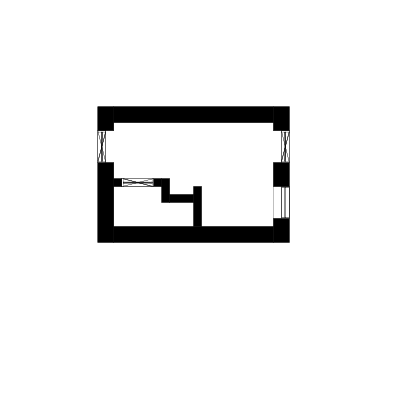
\includegraphics[width=\columnwidth]{fig/scenario1_story_plan.jpg}
    \caption{Gebäudeplan des 3D Modells.}
    \label{fig:Scenario1 Gebäudeplan}
  \end{subfigure}
  \label{fig:Scenario1 komplett}
  \caption{Modell eines Studentenzimmers (verschiedene Darstellungsformen).}
\end{figure}
\subsection*{Beschreibung}
Nun wird ein komplexeres Modell herangezogen.
Zu sehen ist der Plan eines einfachen Hauses mit einem Stockwerk.
Dieses besitzt eine Eingangstür, eine Terassentür neben einem Fenster und eine Tür, die das Badezimmer vom Hauptraum trennt.
Türen und Fenster stellen eine Herausforderung für den Planungsalgorithmus dar, da der Verlauf einer ansonsten durchgängigen Wand dadurch unterbrochen wird und Lücken aufweist.
Details wie Duschen, Betten, Toiletten und ähnliche Komponenten, sind für alle Szenarien dieser Arbeit irrelevant, da diese keinen Effekt auf die Struktur der Wände haben und wurden aus diesem Grund bewusst weggelassen.
Es gibt breite Außen- und dünne Innenwände.
Dafür müssen zwei Wandtypen definiert werden, die jeweils unterschiedliche Wanddicken vorgeben.
Diese entsprechen in ihren Maßen dem Raster, welches das \textit{LEGO System} (siehe Kapitel~\ref{basics}) vorgibt.
Für breite Wände gilt, dass diese immer zwei Noppen breit, mindestens eine Noppe lang und einen Stein hoch sein muss.
Für dünne Wände hingegen gilt eine feste Breite von einer Noppe, ebenfalls eine Mindestlänge von einer Noppe und eine Mindesthöhe von einem Stein.
Beide Wandtypen können nur Höhen beziehungsweise Längen aufweisen, die jeweils einem Vielfachen der Höhe oder Länge des kleinsten Legosteins aufweisen, der zum Bau der Wände verwendet werden soll (hier der 1x1 Stein).
Daraus resultiert ein Raster, welches ebenfalls für die Ausmaße und Positionen der Fenster und Türen einzuhalten ist.
Dieses Raster gilt es, abhängig des ausgewählten Wandtyps, in den Editor zu integrieren, um das Modellieren solcher Gebäude nutzerfreundlich zu gestalten und nicht durch ständiges Messen und Eintragen genauer Positionen oder Maße zu unterbrechen.
\begin{figure}[!ht]
  \centering
  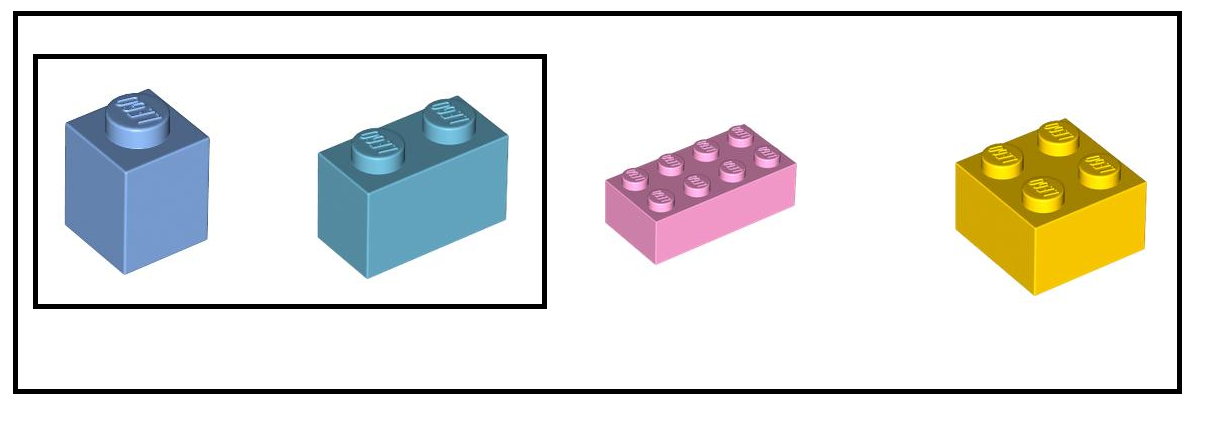
\includegraphics[width=0.6\columnwidth]{fig/scenario1_lego_set.png}
  \caption{LEGO Steintypen für die Innen- und Außenwände. (TODO Bild ist sehr hässlich)}
  \label{fig:Scenario1 Lego Set}
\end{figure}
Nicht nur die Abmessungen der Wände müssen in ein Raster fallen, auch deren Rotation wird in diesem Szenario auf 90\textdegree{} Schritte limitiert. 
Das stellt in diesem Fall eine vertretbare Enschränkung dar, da es ohnehin dem intuitiven Umgang mit LEGO Steinen und gleichzeitig dem Baustil der meisten einfachen Gebäuden entspricht.
\subsection*{Problemstellungen}
\paragraph{Überbindemaß TODO}
Obwohl in dem vorliegenden Modell ausschließlich Einsteinmauerwerke vorgesehen sind, gilt es die in Kapitel \ref{basics:Mauerwerksverband} erläuterte Regel zum Überbindemaß von Bausteinen zu beachten.
Da es sich hierbei aber um LEGO Steine handelt, die wesentlich kleiner sind als die genormten Formate für Ziegelsteine, wird der für das Überbeindemaß vorgesehene Mindestwert von 45mm ignoriert.
Außerdem ist ein Versatz von unter 50\% der Dicke eines Legosteines in den meisten Fällen nicht umsetzbar, da diese nicht frei übereinander gesteckt werden können.
Darum wird für dieses Szenario wird ein Überbindemaß von exakt 50\% der Steindicke verwendet, was den Einschränkungen des Überbindemaßes entspricht, welches einen Mindestversatz von 40\% der Steindicke voraussetzt.
Für die in Abbildung \ref{fig:Scenario1 Lego Set} dargestellten Lego Steine kann mit einem solchen Überbindemaß gleichzeitig auch das vorgesehene Raster des Lego Systems eingehalten werden, da diese alle eine gerade Anzahl an Noppen besitzen.
TODO Bild von dumm gestapelter LEGO Wand zu LEGO Wand mit Überbindemaß.
\begin{itemize}
  \item Wie können Öffnungen berücksichtigt werden?
  \item T-Kreuzungen?
\end{itemize}

\section{Bauplandeduktion eines Gebäudemodells des KIT}\label{scenarios:scenario3}
Um das Konzept nicht nur an eigens modellierten Gebäuden zu evaluieren, werden zusätzlich externe Modelle herangezogen.
Dabei kann sich zum Beispiel an den Beispielprojekten des KIT bedient werden~\cite{KITSAMPLEHOUSE:online}.
TODO Bild von kleinem Hause
TODO überlegen ob eines der beiden riesendinger auch mal ran soll?

\section{Definition von Regelsets}\label{scenarios:scenario4}
\subsection*{Beschreibung}
\subsection*{Problemstellungen}
\begin{itemize}
  \item Wie können Regelsets ohne Code vorgegeben werden? Also in welchem Format.
  \item In welcher Weise werden die Regeln dann angewendet etc?
\end{itemize}